\documentclass{article}

\usepackage{minted}
\usepackage{xcolor}
\usepackage{tikz}
\usetikzlibrary{quotes, calc}

\usepackage{booktabs}

\title{EE 450 Wireshark Lab: DHCP Report}
\author{Shangning Xu}

\begin{document}

\maketitle
\newpage

\begin{abstract}
    We answer assigned questions and discuss observed behaviors of DHCP in this report for the Wireshark Lab: DHCP.
\end{abstract}

\section{Answers to Questions}

\begin{enumerate}
    \item UDP, as shown in the following packet. This is the first DHCP packet in our capture.
\begin{minted}[breaklines, escapeinside=!!]{text}
Frame 12: 342 bytes on wire (2736 bits), 342 bytes captured (2736 bits) on interface en0, id 0
Ethernet II, Src: Apple_9b:a0:49 (98:01:a7:9b:a0:49), Dst: Broadcast (ff:ff:ff:ff:ff:ff)
Internet Protocol Version 4, Src: 0.0.0.0, Dst: 255.255.255.255
!\colorbox{yellow}{User Datagram Protocol}!, Src Port: 68, Dst Port: 67
Dynamic Host Configuration Protocol (Discover)
\end{minted}

    \item The timing diagram is shown below. Each packet is labeled with its source and destination's IP address and port number. The port numbers are the same as the ones in the example given in the lab assignment.
    
    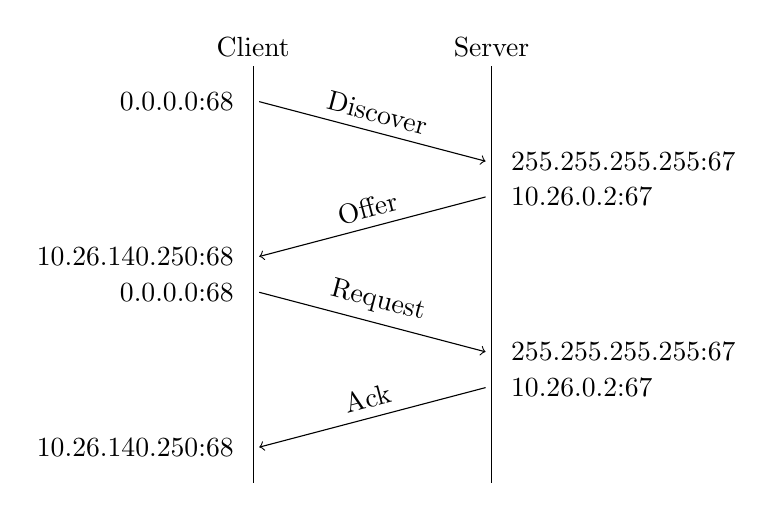
\begin{tikzpicture}
        \draw (0, 0) -- (0, 35ex) node [above] {Client} (20ex, 0) -- ++(0, 35ex) node [above] {Server};
        \node (c discover) [label=left:0.0.0.0:68] at (0ex, 32ex) {};
        \node (s discover) [label=right:255.255.255.255:67] at (20ex, 27ex) {};
        \draw [->] ($(c discover) + (0.5ex, 0)$) -- node [sloped, above] {Discover} ($(s discover) - (0.5ex, 0)$);

        \node (s offer) [label=right:10.26.0.2:67] at (20ex, 24ex) {};
        \node (c offer) [label=left:10.26.140.250:68] at (0ex, 19ex) {};
        \draw [->] ($(s offer) - (0.5ex, 0)$) -- node [sloped, above] {Offer} ($(c offer) + (0.5ex, 0)$);

        \node (c request) [label=left:0.0.0.0:68] at (0ex, 16ex) {};
        \node (s request) [label=right:255.255.255.255:67] at (20ex, 11ex) {};
        \draw [->] ($(c request) + (0.5ex, 0)$) -- node [sloped, above] {Request} ($(s request) - (0.5ex, 0)$);

        \node (s ack) [label=right:10.26.0.2:67] at (20ex, 8ex) {};
        \node (c ack) [label=left:10.26.140.250:68] at (0ex, 3ex) {};
        \draw [->] ($(s ack) - (0.5ex, 0)$) -- node [sloped, above] {Ack} ($(c ack) + (0.5ex, 0)$);
    \end{tikzpicture}

    \item 98:01:a7:9b:a0:49, as shown in the packet in the answer to Question 1:
\begin{minted}[breaklines, escapeinside=!!]{text}
Ethernet II, Src: Apple_9b:a0:49 (!\colorbox{yellow}{98:01:a7:9b:a0:49}!), Dst: Broadcast (ff:ff:ff:ff:ff:ff)
\end{minted}

    \item The DHCP Message Type field. This is the field's value for a DHCP discover message:
\begin{verbatim}
Option: (53) DHCP Message Type (Discover)
    Length: 1
    DHCP: Discover (1)
\end{verbatim}
    And this is for a DHCP request message:
\begin{verbatim}
Option: (53) DHCP Message Type (Request)
    Length: 1
    DHCP: Request (3)
\end{verbatim}

    \item For the first four messages the Transaction-ID is 0xefaf8ff2 and for the second set 0xefaf8ff3, as shown in the following list of DHCP packets. The purpose of the Transaction-ID field is for the server to differentiate client requests.
    
    \begin{tabular}{@{}lllll@{}}
    \toprule
    No.  & Time      & Source    & Destination     & Info                                      \\ \midrule
    12   & 9.868620  & 0.0.0.0   & 255.255.255.255 & DHCP Discover - Transaction ID \colorbox{yellow}{0xefaf8ff2} \\
    13   & 10.924357 & 10.26.0.2 & 10.26.140.250   & DHCP Offer    - Transaction ID 0xefaf8ff2 \\
    21   & 11.929991 & 0.0.0.0   & 255.255.255.255 & DHCP Request  - Transaction ID 0xefaf8ff2 \\
    22   & 11.934212 & 10.26.0.3 & 10.26.140.250   & DHCP ACK      - Transaction ID 0xefaf8ff2 \\
    24   & 11.935314 & 10.26.0.2 & 10.26.140.250   & DHCP ACK      - Transaction ID 0xefaf8ff2 \\
    1244 & 24.025924 & 0.0.0.0   & 255.255.255.255 & DHCP Request  - Transaction ID \colorbox{yellow}{0xefaf8ff3} \\
    1248 & 24.028606 & 10.26.0.2 & 10.26.140.250   & DHCP ACK      - Transaction ID 0xefaf8ff3 \\
    1249 & 24.029635 & 10.26.0.3 & 10.26.140.250   & DHCP ACK      - Transaction ID 0xefaf8ff3 \\
    1250 & 24.029640 & 10.26.0.2 & 10.26.140.250   & DHCP ACK      - Transaction ID 0xefaf8ff3 \\
    1251 & 24.030677 & 10.26.0.3 & 10.26.140.250   & DHCP ACK      - Transaction ID 0xefaf8ff3 \\ \bottomrule
    \end{tabular}

    \item The source and destination IP addresses for each DHCP message have been indicated in the timing diagram in the answer to Question 2.
    
    \item The DHCP server's IP address is 10.17.14.11, indicated in the following DHCP offer message:
\begin{minted}[breaklines, escapeinside=!!]{text}
Option: (53) DHCP Message Type (Offer)
Option: (54) DHCP Server Identifier (!\colorbox{yellow}{10.17.14.11}!)
Option: (51) IP Address Lease Time
Option: (1) Subnet Mask (255.255.0.0)
Option: (3) Router
Option: (6) Domain Name Server
Option: (15) Domain Name
Option: (119) Domain Search
Option: (255) End
\end{minted}

    \item The DHCP server offered me the address 10.26.140.250 in the DHCP offer message, as shown in the following content of the DHCP offer message:
\begin{minted}[breaklines, escapeinside=!!]{text}
Message type: Boot Reply (2)
Hardware type: Ethernet (0x01)
Hardware address length: 6
Hops: 2
Transaction ID: 0xefaf8ff2
Seconds elapsed: 0
Bootp flags: 0x0000 (Unicast)
Client IP address: 0.0.0.0
Your (client) IP address: !\colorbox{yellow}{10.26.140.250}!
Next server IP address: 0.0.0.0
Relay agent IP address: 10.26.0.2
Client MAC address: Apple_9b:a0:49 (98:01:a7:9b:a0:49)
Client hardware address padding: 00000000000000000000
Server host name not given
Boot file name not given
Magic cookie: DHCP
\end{minted}

    \item The \texttt{giaddr} field having the value of 0.0.0.0 in the offer message indicates the absence of a relay agent. There is a relay agent with an IP address of 10.26.0.2 in my experiment, as shown in the DHCP offer message in the answer to question 8.

    \item The router and subnet mask fields in the DHCP offer message tells the client what IP addresses are not in the subnet and where to deliver datagrams bound for the router or those IP addresses not in the subnet.

    \item The client accepts this IP address, as shown in the option "Requested IP Address" field in the DHCP request message, which is reproduced below:
\begin{verbatim}
Option: (50) Requested IP Address (192.168.1.101)
    Length: 4
    Requested IP Address: 192.168.1.101
\end{verbatim}

    \item The lease time allows the DHCP server to reuse IP addresses whose leases have expired. Otherwise, the number of available IP addresses will be quickly exhausted because the server doesn't know when an IP address can be reused.
    
    The lease time is one day, as shown below in the DHCP offer message:
\begin{verbatim}
Option: (51) IP Address Lease Time
    Length: 4
    IP Address Lease Time: (86400s) 1 day
\end{verbatim}

    \item The DHCP release message allows a client to release its IP address back to the server. The server doesn't acknowledge receipt of the client's release message. If the release message is lost, the server will not know that the client has released its IP address, and the IP address won't be reused until the lease expires.
    
    \item Yes, the following ARP packets are exchanged during the DHCP packet-exchange period:

    \begin{tabular}{@{}lllll@{}}
        \toprule
        No. & Time      & Source          & Destination     & Info                               \\ \midrule
        25  & 11.936485 & Apple\_9b:a0:49 & Apple\_9b:a0:49 & Who has 10.26.140.250? (ARP Probe) \\
        28  & 12.254749 & Apple\_9b:a0:49 & Broadcast       & Who has 10.26.140.250? (ARP Probe) \\
        29  & 12.256693 & Apple\_9b:a0:49 & Apple\_9b:a0:49 & Who has 10.26.140.250? (ARP Probe) \\
        30  & 12.575018 & Apple\_9b:a0:49 & Broadcast       & Who has 10.26.140.250? (ARP Probe) \\
        31  & 12.579275 & Apple\_9b:a0:49 & Apple\_9b:a0:49 & Who has 10.26.140.250? (ARP Probe) \\
        32  & 12.900117 & Apple\_9b:a0:49 & Broadcast       & ARP Announcement for 10.26.140.250 \\
        36  & 13.225234 & Apple\_9b:a0:49 & Broadcast       & ARP Announcement for 10.26.140.250 \\
        41  & 13.550478 & Apple\_9b:a0:49 & Broadcast       & ARP Announcement for 10.26.140.250 \\ \bottomrule
    \end{tabular}

    The client first broadcast ARP probes to find out if the IP address was already in use. Receiving no responses for ARP probes, the client broadcast ARP announcements so that other hosts could update their ARP tables.
\end{enumerate}


\section{Conclusion}

My experiment in performed in the university-wide network ``USC Secure Wireless'' under macOS 12.1. The client-server interaction differs from the one in the textbook in the following ways:

\begin{itemize}
    \item There are two relay agents present in the network at 10.26.0.2 and 10.26.0.3. Only 10.26.0.2 responded to our DHCP discover message, while both responded to our DHCP request message.
    \item The DHCP offer message was unicast, rather than broadcast as in the textbook, due to the bootp flags unset in the DHCP request message.
\end{itemize}

Wireshark is mostly easy to use. However, the algorithm that groups messages into ``conversations'' is not intelligent enough. Messages seem to be grouped into conversations solely based on the source and destination IP or MAC addresses, which fails spectacularly in the case of the DHCP protocol. DHCP's four messages should have been grouped into one message, but not due to different IP addresses. On Wireshark's GUI, this can be observed in the ``No.'' column of the packet list pane, as shown in Figure~\ref{fig:wireshark-conversations}. DHCP discover and request messages across DHCP transactions are grouped into one conversation because they have the same source (0.0.0.0) and destination (255.255.255.255) IP addresses, while offer and acknowledgment messages are grouped into another.

\begin{figure}[tb]
    \includegraphics[width=\linewidth]{img/wireshark-conversations.png}
    \caption{Wireshark packet list pane. Grey lines in the red box are how Wireshark (confusingly) groups messages and displays conversations.}
    \label{fig:wireshark-conversations}
\end{figure}

\end{document}
